\documentclass[10pt,letterpaper]{article}
\usepackage[letterpaper,top=1in,bottom=1in,left=1.05in,right=1.05in]{geometry}
\usepackage[T1]{fontenc}
\usepackage{amsmath,amsthm}
\usepackage{txfonts}
\usepackage[expansion=false]{microtype}
\usepackage{parskip}
\usepackage{tikz}
\usetikzlibrary{arrows.meta,positioning,calc,fit}
\usepackage{booktabs,tabularx,array}
\usepackage{caption}
\usepackage{float}
\usepackage{xcolor}
\usepackage{url}
\usepackage[hidelinks]{hyperref}

\captionsetup{font=small,labelfont=bf,labelsep=period}
\setlength{\parskip}{0.5em}
\linespread{1.03}
\pagestyle{plain}
\emergencystretch=1.5em

\makeatletter
\renewcommand\section{\@startsection{section}{1}{\z@}{-1.3em}{0.45em}{\normalfont\large\bfseries}}
\renewcommand\subsection{\@startsection{subsection}{2}{\z@}{-0.9em}{0.25em}{\normalfont\normalsize\bfseries}}
\renewcommand\thesection{\arabic{section}.}
\renewcommand\thesubsection{\arabic{section}.\arabic{subsection}}
\renewcommand\@seccntformat[1]{\csname the#1\endcsname\ }
\makeatother

\theoremstyle{plain}
\newtheorem{theorem}{Theorem}
\newtheorem{lemma}{Lemma}
\newtheorem{proposition}{Proposition}
\theoremstyle{definition}
\newtheorem{definition}{Definition}

\newcommand{\ak}{\mathsf{ak}}
\newcommand{\ask}{\mathsf{ask}}
\newcommand{\nk}{\mathsf{nk}}
\newcommand{\rivk}{\mathsf{rivk}}
\newcommand{\ivk}{\mathsf{ivk}}
\newcommand{\ovk}{\mathsf{ovk}}
\newcommand{\rk}{\mathsf{rk}}
\newcommand{\fvk}{\mathsf{FVK}}
\newcommand{\Gor}{\mathcal{G}}
\newcommand{\ytilde}{\tilde{y}}
\newcommand{\fn}[1]{\texttt{#1}}
\newcommand{\st}[1]{\textsf{#1}}
\newcommand{\tbd}[1]{\textcolor{red}{[#1]}}
\newcommand{\TLCa}{352}\newcommand{\TLCb}{52{,}423}\newcommand{\TLCc}{327{,}390}
\newcommand{\TLCda}{2{,}406}\newcommand{\TLCdl}{2{,}124{,}904}\newcommand{\TLCdb}{856{,}632}\newcommand{\TLCdc}{13{,}467{,}219}

\begin{document}

\begin{center}
{\Large\bfseries Cloakroom: A Dark Pool for Shielded Zcash\\[0.2em] with Scriptless Atomic Settlement}\\[1.1em]
{\normalsize Chris Gachau}\\[0.25em]
{\small October 2026}
\end{center}

\vspace{0.3em}
\begin{quote}
\small
\textbf{Abstract.} Every route out of shielded Zcash today passes through a transparent address
held by an exchange, a bridge or an intent network, which publishes amounts and timing and can
hold funds. Cloakroom trades shielded ZEC against tokens on an EVM chain without either. The two
parties split the spend authorizing key of a fresh Ironwood address into additive shares, and
the counterparty's tokens sit in an escrow whose two exits each publish one share. We give a
timing model with bounded inclusion delay, finality lag and a budget of reorganizations, and
prove three things. An honest taker loses at most a small premium and is never held hostage while she stays online
through her claim. An honest maker
never loses funds if he comes online once in a stated window, which any protocol that pays the
taker's unilateral exit on the EVM chain without observing Zcash must require. A passive observer learns nothing that links the two chains beyond timing and the wallet
fingerprint the transactions share. Model checking the protocol in TLA$^+$ found that a refund
which is included but not yet final can be reorganized into a theft, and, at a second parameter
point, was consistent with the budget every share-revealing transaction needs, which a reviewer of an
earlier version derived; our checked points all have $D=F$, so the budget's form rests on its proof. Measuring 30 days of Zcash mainnet shows that timing is the
binding privacy constraint. A swap transaction that is not delayed hides among almost no others.
A natural count-gated delay lets an observer who knows the policy guess the transaction with
probability 0.18 in the median case and above 0.85 in one case in ten; the delay our wallet
uses keeps it near 1.4\% per delayed transaction (median, for an observer who samples its
posterior) at an average of 2.6 hours per delayed step; by a union bound over a swap's four
anchored transactions, a swap is linked with probability at most about 6\%, and more if the
observer matches every wallet setting.
The implementation passes eighteen two-party scenarios, including injected reorganizations, an
impostor maker, malicious quotes and a funding mined after the maker's refund. On Zcash testnet and Base Sepolia the final escrow has settled swaps, and every
Zcash transaction was fully shielded.
\end{quote}

\section{Introduction}

Zcash~\cite{zerocash,spec} offers two kinds of value. Transparent value is public, as in
Bitcoin~\cite{bitcoin}. Shielded value is held as encrypted notes, and a fully shielded transaction
shows an observer only that it happened and what fee it paid. Most shielded ZEC is now in
the Ironwood pool introduced by NU6.3 in July 2026~\cite{zip258}.

Shielded value stays private only while it stays shielded. Each crossing between transparent
and shielded value publishes an amount and a time, and matching crossings has linked a large
share of shielded activity to transparent addresses~\cite{kappos,quesnelle,biryukov}; similar
methods recently linked 17.65\% of Railgun withdrawals on Ethereum~\cite{railgun}. On mainnet,
51\% of Ironwood transactions in the last 30 days touched a transparent address
(Section~8.2). Exchange is where this happens: most exchanges withdraw ZEC only to transparent
addresses; NEAR Intents supports ZEC on transparent addresses only~\cite{nearchains}; and Maya
and THORChain hold ZEC in transparent vaults. Each route also adds a custodian. A user reported
a \$589{,}000 payout from a ZEC swap held in a compliance review for more than fifty
days~\cite{freeze}, and on October~1, 2026 NEAR Intents was exploited for about \$3.8 million
before pausing and, according to reports, recovering the funds~\cite{nearexploit}.

Hash-locked atomic swaps~\cite{nolan,herlihy} remove the custodian but need scripts, which
Zcash's shielded pools lack; on transparent outputs, the shared hash links both legs~\cite{xcat}.
Monero, which also lacks scripts, swaps by locking its leg to a key split between the
parties~\cite{gugger,athanor}. Cloakroom brings this approach to Orchard-protocol keys, which the
Ironwood pool uses, and adds what a deployable venue needs. We make five contributions.
\begin{itemize}\setlength\itemsep{0.1em}
\item \textbf{A protocol.} A swap between shielded ZEC and any EVM token whose Zcash leg is
ordinary fully shielded transactions. Claims need Ready and are committed before they are
revealed, payments are pulled, and a punish window removes the hostage case
(Section~4).
\item \textbf{A model and proofs.} A timing model with inclusion delay $D$, finality lag $F$
and $R$ reorganizations, giving every share-revealing transaction the budget $(R+1)D + RF$.
Proofs of taker safety without hostage, of maker safety under a liveness condition, and that the
condition is needed whenever the taker's unilateral exit is paid on the EVM chain, which does not
observe Zcash (Sections~3 and~5).
\item \textbf{Mechanized verification.} A TLA$^+$ model checked by TLC at three small parameter points, $(D,F,R) \in \{(1,1,1), (2,2,1), (2,2,2)\}$,
in which removing any of the rules R2c--R3l or L$_M$, or shortening either budget by one step,
yields a concrete attack.
Symbolic execution, mutation testing, static analysis and stateful fuzzing of the escrow
(Section~6).
\item \textbf{A measured privacy analysis.} A simulation argument for passive observers, anonymity
sets measured on 30 days of Zcash mainnet, and the posterior of an observer who knows the delay
policy, which determines the policy our wallet uses (Section~8).
\item \textbf{An implementation.} Run in eighteen two-party scenarios, two of them with injected
reorganizations, one with an impostor maker, two with malicious quotes and one with a late funding, and on public test networks (Section~9).
\end{itemize}

We use ``dark pool'' in its trading sense: a venue without pre-trade transparency. Requests and
quotes in Cloakroom travel encrypted, and only the executed price becomes public. Unlike an
exchange-run dark pool, Cloakroom has no central matching; it is bilateral request-for-quote
between a taker and a market maker. The taker is anonymous; the maker's EVM address is public.

\section{Background}

\textbf{Orchard keys.} Orchard~\cite[\S4.2.3]{spec} works over Pallas,
$E_p: y^2 = x^3 + 5$, with prime group order $q$. A spending key yields a spend authorizing key
$\ask \in \mathbb{F}_q^*$, a nullifier key $\nk \in \mathbb{F}_p$ and a randomness
$\rivk \in \mathbb{F}_q$. The spend validating key is $\ak = [\ask]\Gor$, where $\Gor$ is the
RedPallas spend-authorization base point. A full viewing key $(\ak, \nk, \rivk)$ encodes $\ak$
by its $x$-coordinate~\cite[\S5.6.4.4]{spec}, so key generation fixes $\ytilde(\ak)=0$, negating
$\ask$ if needed. From the full viewing key derive the incoming viewing key
$\ivk = \mathsf{Commit}^{\ivk}_{\rivk}(\mathsf{Extract}(\ak),\nk) \notin \{0,\bot\}$, an outgoing
viewing key $\ovk$, and mutually unlinkable diversified addresses.

\textbf{Spending.} A transaction is a set of actions, each pairing a spend and an output. To
spend, one picks a fresh $\alpha$, publishes $\rk = \ak + [\alpha]\Gor$, and signs the ZIP~244
sighash~\cite{zip244} with RedPallas under $\ask + \alpha$. A Halo~2 proof~\cite{halo2} shows
that $\rk$ randomizes the $\ak$ of the spent note's address, that the note is in the commitment
tree, and that the nullifier is correct. An action publishes a value commitment, nullifier,
$\rk$, note commitment, ephemeral key and ciphertexts.

\textbf{Ironwood and NU7.} A soundness flaw in the Orchard action circuit was disclosed in May
2026. NU6.2 (June 2026) fixed the circuit and re-enabled Orchard. NU6.3 (July 28, 2026) then
introduced the Ironwood pool, with its own note-commitment tree, nullifier set and value pool, and
limited the Orchard pool to withdrawals through a turnstile~\cite{zip258}. Ironwood keeps Orchard's keys and addresses, and one incoming
viewing key scans both pools~\cite{zip326}. NU7 (testnet since October~4, 2026) shortens blocks to
25~s and keeps the transaction format~\cite{zip259}. A partially created transaction
(PCZT)~\cite{zip374} separates construction, proving and signing, so that a spend can be signed
by a key that no wallet holds; Zcash's FROST support uses the same interface~\cite{frost,zip312}.

\textbf{The EVM chain.} We use Base, an Ethereum rollup. Its transactions are ordered by a
sequencer; a transaction deposited through the \fn{OptimismPortal} contract on Ethereum must be
included within the sequencing window, 3{,}600 Ethereum blocks or about 12~hours, which still
holds after Base's May 2026 Azul upgrade~\cite{basereliab,opforced}. We measured the lag of
Base's finalized head at 846--890~s on mainnet and 1{,}058--1{,}102~s on Sepolia.

\section{Model and Goals}

\textbf{Parties.} A taker $T$ holds shielded ZEC and wants $u$ tokens; a maker $M$ holds the
tokens. A probabilistic polynomial-time adversary $\mathcal{A}$ statically corrupts at most one of
them. It schedules transactions within the bounds below and observes all public data. It may also
crash the honest party at any time and restore it later; the party's state persists. We assume
one thing about crashes:
\begin{itemize}\setlength\itemsep{0.05em}
\item \textbf{(H) Continuity.} An honest party that has broadcast a transaction publishing or
committing to its share stays online until that transaction's effect is final. For the taker this
spans from her first \fn{commitClaim} to the finality of her claim, or of the maker's refund.
\end{itemize}
Hash-locked swaps make the same assumption about the party that reveals a preimage. Without it a
taker who commits and then goes offline past the reveal window cannot claim, and a malicious maker
need never refund, so her ZEC stays locked. The commit signature has no validity interval, so a
commit that reverted can be replayed later; under (H) this is harmless, because the taker is
online and reveals within $W$. Rule L$_M$ (Section~4) adds one requirement for the maker.

\textbf{Clock.} A party measures time by the timestamp of the latest EVM block it has seen, which
we write $\tau$. Block timestamps are monotone. The bounds below are stated in this clock, so a
party's view lag and the sequencer's timestamp drift are part of $D$.

\textbf{EVM ledger.}
\begin{itemize}\setlength\itemsep{0.05em}
\item \textbf{(E1) Bounded inclusion.} An honest transaction broadcast at $\tau$ is included in a
block with timestamp at most $\tau + D$, unless a reorganization drops it. If its preconditions
fail at inclusion, it reverts.
\item \textbf{(E2) Finality and reorganizations.} At $\tau$, blocks with timestamp at most
$\tau - F$ are final. A younger block may be reorganized away; its transactions are dropped, and
the sender must re-send them. $\mathcal{A}$ reorganizes at most $R$ times per swap.
\item \textbf{(E3) Public calldata.} $\mathcal{A}$ learns the calldata of every broadcast
transaction, \emph{including one that later reverts or is reorganized away}.
\end{itemize}
Each reorganization can come just before finality, after which the re-sent copy again needs up
to $D$. A transaction that must survive $R$ reorganizations therefore needs the budget
\[
B_R = (R+1)D + RF.
\]

\textbf{Zcash ledger.}
\begin{itemize}\setlength\itemsep{0.05em}
\item \textbf{(Z1) Persistence.} A transaction with $k_Z$ confirmations is reverted with
probability at most $\varepsilon_Z$. We do not quantify $\varepsilon_Z$; a deployment should
choose $k_Z$ from the value at risk, and in blocks rather than minutes, since NU7 shortens the
block interval.
\item \textbf{(Z2) Liveness.} A valid honest transaction is mined within $\Delta_Z$, which
includes any expiry (40 blocks after its target height) and re-send.
\end{itemize}

\textbf{Cryptographic assumptions.}
\begin{itemize}\setlength\itemsep{0.05em}
\item Discrete logarithms are hard on Pallas.
\item Halo~2 with the Ironwood action circuit (the circuit as fixed in NU6.2) is knowledge-sound
and zero-knowledge.
\item RedPallas spend authorization is unforgeable for keys rerandomized by additive offsets known
to the adversary~\cite{spec,rerandfrost}. Zcash relies on the same property, since every spender
chooses its own randomizer $\alpha$.
\item The Fiat--Shamir Schnorr proofs of knowledge are straight-line extractable in the
algebraic group and random oracle models~\cite{agm}.
\item keccak256 and BLAKE2b behave as random oracles.
\item ECDSA on secp256k1 is EUF-CMA.
\item ChaCha20-Poly1305 is a secure AEAD (IND-CPA and INT-CTXT), and Gap-DH holds on Pallas.
\item Ironwood transactions of the same \emph{shape} are indistinguishable to an observer without
the keys. The shape is every public field outside the cryptographic payload: the number of
actions, the fee, \texttt{lock\_time}, the expiry height relative to the mined height, and the
block. Section~8.2 measures how large these classes are.
\item Token transfers eventually succeed. A token issuer that blocks an address forever is an
issuer risk, which no protocol over that token can remove.
\end{itemize}

\textbf{Goals.} Let $v$ be the ZEC funded to the joint address and $u$ the tokens escrowed.
\begin{definition}[Taker safety]
An honest $T$ ends in one of three states: (i) she never funded, and lost at most the premium
$\pi$ (Section~5); (ii) she is credited
$u - f_r$, where $f_r$ is the relayer fee; or (iii) she can spend the joint note, or has spent
it. In particular, no execution leaves her ZEC spent by someone else while she is uncredited.
\end{definition}
\begin{definition}[No hostage]
An honest $T$ who funded reaches (ii) or (iii) within bounded time, without any action by $M$.
\end{definition}
\begin{definition}[Maker safety]
An honest $M$ ends either refunded, or with $T$ credited and $M$ able to spend a final joint
note of value at least $v$.
\end{definition}
\begin{definition}[Unlinkability]
A passive observer of both chains cannot distinguish a swap's Zcash transactions from other
Ironwood transactions of the same shape in the same blocks.
\end{definition}

\section{The Protocol}

\subsection{Key setup}
Quotes and requests travel over Zcash memos (Section~7); here we give the keys.
\begin{enumerate}\setlength\itemsep{0.1em}
\item $T$ samples $a \leftarrow \mathbb{F}_q^*$ and a seed $s_T$; $M$ samples $b$ and $s_M$, all fresh
per request. They exchange $A=[a]\Gor$ and $B=[b]\Gor$, each with a Schnorr proof of knowledge.
Each proof's challenge binds the request identifier $\mathsf{sid}$ and the party's role, and each
party verifies the other's proof before use.
\item $T$ commits to $s_T$ in her request and opens it in her acceptance. Both derive
$\nk = H_{\mathbb{F}_p}(\mathsf{dom}_{\nk},\mathsf{sid},s_T,s_M)$ and
$\rivk = H_{\mathbb{F}_q}(\mathsf{dom}_{\rivk},\mathsf{sid},s_T,s_M)$ with personalized,
length-prefixed BLAKE2b-512 and distinct domain tags.
\item If $\ytilde(A+B)=1$, both parties negate their shares and points. This is deterministic, so
$\ak = A+B$ then has $\ytilde = 0$. The escrow stores the normalized points; a proof of knowledge
of $\log A$ is also one of $\log(-A)$.
\item Both check that $\fvk_J = (\ak,\nk,\rivk)$ is a valid full viewing key, and derive the
external address at index~0 as $\mathsf{addr}_J$, encoded with an Orchard receiver only. Value
sent there enters Ironwood.
\end{enumerate}
Both parties can view $\mathsf{addr}_J$; spending needs $a+b$. The proofs of knowledge prevent the
rogue-key choice $B = [b']\Gor - A$~\cite{musig}. ZIP~2005~\cite{zip2005} specifies how wallets
derive keys so that notes stay recoverable after a quantum break; both of its branches start from
a spending key or a quantum spending key. A joint key has neither, so joint notes are not
quantum-recoverable. Consensus does not check how a full viewing key was derived, and a joint
note lives only until the swap settles.

\subsection{Escrow}
For each swap the escrow stores the maker, the taker's payout address, the token, $u$, $f_r$, $A$
and $B$, deadlines $t_0 < t_1 < t_2$ and a reveal window $W$. The swap identifier is
$\mathrm{keccak}(\mathit{maker}, \mathit{salt})$, so it is scoped to the maker. The salt is
$H(\mathsf{dom}_{\mathit{salt}}, \mathsf{sid}, s_T, s_M)$. The request identifier $\mathsf{sid}$
travels in memo envelopes, so a salt derived from it alone would let anyone who later obtains a
party's viewing key find the swap's escrow. The state machine is in Table~\ref{tab:fsm}.

\begin{table}[H]
\centering\small
\begin{tabularx}{\linewidth}{@{}l l X@{}}
\toprule
\textbf{Call} & \textbf{From} $\to$ \textbf{to} & \textbf{Condition and effect}\\
\midrule
\fn{open} & -- $\to$ \st{Open} & By $M$. $A$ and $B$ on the curve and canonical, $f_r \le u$, $\tau < t_0 < t_1 < t_2$. Pulls $u$ tokens and rejects tokens that deliver less.\\
\fn{setReady} & \st{Open} $\to$ \st{Ready} & By $M$, $\tau < t_0$.\\
\fn{commitClaim} & \st{Ready} $\to$ \st{Locked} & ECDSA signature by the payout key over (escrow, chain id, swap id, $c$, relayer), $\tau < t_1$. Stores $c = \mathrm{keccak}(\mathit{id}, a)$; reveals nothing.\\
\fn{commitClaim} & \st{Open}/\st{Ready} $\to$ \st{Locked} & Same signature, $\tau \ge t_2$ (punish path).\\
\fn{claim}$(a)$ & \st{Locked} $\to$ \st{Claimed} & Anyone. $\tau < \mathit{lockedAt} + W$, $\mathrm{keccak}(\mathit{id},a)=c$, $[a]\Gor = A$. Credits $u-f_r$ to the payout and $f_r$ to the committed relayer. No external calls.\\
\fn{refund}$(b)$ & \st{Open} $\to$ \st{Refunded} & $\tau < t_0$, $[b]\Gor = B$. Credits $u$ to $M$. No external calls.\\
\fn{refund}$(b)$ & \st{Open}/\st{Ready} $\to$ \st{Refunded} & $t_1 \le \tau < t_2$.\\
\fn{refund}$(b)$ & \st{Locked} $\to$ \st{Refunded} & $\tau \ge \mathit{lockedAt} + W$.\\
\fn{withdraw} & -- & Anyone; pays an owner's credit. Reveals nothing.\\
\bottomrule
\end{tabularx}
\caption{Escrow state machine. \st{Claimed} and \st{Refunded} are terminal.}
\label{tab:fsm}
\end{table}

The Pallas check uses Jacobian coordinates and a projective comparison with the stored point. It
rejects scalars equal to $0$ or at least $q$, non-canonical coordinates, and the point at
infinity. The escrow verifies a Pallas point directly, so unlike the Monero--Ethereum
construction~\cite{athanor,mrl10} it needs no cross-curve equality proof.

\subsection{Settlement and wallet rules}
\begin{figure}[H]
\centering
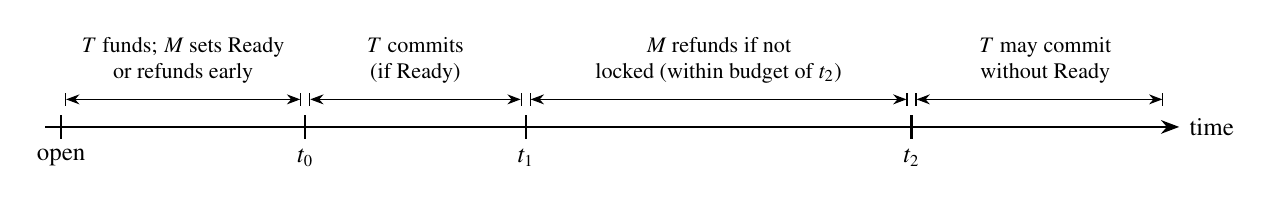
\begin{tikzpicture}[font=\small, >=Stealth]
\draw[thick,->] (0,0) -- (14.4,0) node[right]{time};
\foreach \x/\l in {0.2/open, 3.3/$t_0$, 6.1/$t_1$, 11.0/$t_2$} { \draw[thick] (\x,0.15) -- (\x,-0.15) node[below]{\l}; }
\node[align=center, font=\footnotesize] at (1.75,0.85) {$T$ funds; $M$ sets Ready\\or refunds early};
\node[align=center, font=\footnotesize] at (4.7,0.85) {$T$ commits\\(if Ready)};
\node[align=center, font=\footnotesize] at (8.55,0.85) {$M$ refunds if not\\locked (within budget of $t_2$)};
\node[align=center, font=\footnotesize] at (12.7,0.85) {$T$ may commit\\without Ready};
\draw[|<->|, thin] (0.25,0.35) -- (3.25,0.35);
\draw[|<->|, thin] (3.35,0.35) -- (6.05,0.35);
\draw[|<->|, thin] (6.15,0.35) -- (10.95,0.35);
\draw[|<->|, thin] (11.05,0.35) -- (14.2,0.35);
\end{tikzpicture}
\caption{Deadlines. After a commit, $T$ reveals within $W$; after $W$, $M$ may refund a lock that was never revealed.}
\end{figure}

\textbf{Happy path.}
\begin{enumerate}\setlength\itemsep{0.1em}
\item $M$ opens the escrow.
\item Once \fn{open} is final, $T$ funds $v + f$ ZEC to $\mathsf{addr}_J$ in a fully shielded
transaction.
\item After $k_Z$ confirmations, $M$ sets Ready.
\item $T$ commits; once the lock is final, she reveals $a$ by submitting \fn{claim}$(a)$, waits
for the claim to be final, and withdraws.
\item $M$ reads $a$, signs a spend of the joint note under $(a+b)+\alpha$ through PCZT, and sweeps
it to himself with $\ovk = \bot$ and no change to $\mathsf{addr}_J$.
\end{enumerate}
In a refund, $b$ is published and $T$ sweeps the note back the same way.

\textbf{Relayer.} The payout address should hold no ETH, since funding it would link it to the
funder. \fn{commitClaim} therefore names a relayer, who submits the transactions and receives
$f_r$. \fn{claim} is permissionless and pays the committed relayer whoever submits it. A relayer
that receives $a$ could withhold it and publish it after the window closes; $T$ would then lose
both legs. Rule R2r prevents this with a fallback: if the relayer has not broadcast the claim within
a hand-off time $D_h$ (part of $D$), $T$ submits it herself, from any funded address, or through a second relayer. The
budget $B_R$ is counted from the hand-off. With the fallback, a relayer can cost $T$ gas and
some privacy but not funds. Without it, the relayer is trusted for safety. Our implementation
self-relays: the taker holds the relayer key.

Table~\ref{tab:rules} lists the wallet rules. They are part of the protocol: the proofs in
Section~5 depend on them. Section~6 shows an attack when any of R2c, R2r, R3e, R3d, R3l or L$_M$
is removed. R1 and R1b protect the taker's funding against a misconfigured or late escrow, R1q against windows the maker chooses, and R4
protects against a later compromise of the device; the model does not exercise these three.

\begin{table}[H]
\centering\small
\begin{tabularx}{\linewidth}{@{}l l X@{}}
\toprule
\textbf{Rule} & \textbf{Party} & \textbf{Statement}\\
\midrule
R1 & $T$ & Fund only after \fn{open} is final and every stored parameter equals the quote.\\
R1q & $T$ & Accept a quote only if $W > F + B_R$, computed with $T$'s own $D$, $F$ and $R$, and $t_2 - \mathit{open} \le H$ for a horizon $H$ that $T$ chooses. The escrow enforces neither.\\
R1b & $T$ & Fund only if $\tau + \Delta_{\mathit{fund}} < t_0$, where $\Delta_{\mathit{fund}}$ covers $k_Z$ confirmations at a high percentile of block intervals (block times are random), plus $D$ for \fn{setReady}.\\
R2c & $T$ & Commit only once Ready is final and $\tau + B_R < t_1$; or from $t_2$ if the state is \st{Open} or \st{Ready}. (A late commit reverts and reveals only $c$.)\\
R2r & $T$ & Reveal $a$ only once the lock is final and $\tau + B_R < \mathit{lockedAt} + W$, with $\tau$ the hand-off time. Re-send the claim whenever it is dropped; fall back to self-submission if the relayer has not broadcast it.\\
R3e & $M$ & Refund early only in \st{Open} with no sufficient note, after $T$'s R1b funding window has closed. Once $b$ is public, never set Ready.\\
R3d & $M$ & Refund after $t_1$ only if a final block with timestamp $\ge t_1$ shows \st{Open} or \st{Ready}, and $\tau + B_R < t_2$. Re-send whenever dropped.\\
R3l & $M$ & Refund a lock only if a final block with timestamp $\ge \mathit{lockedAt}+W$ shows \st{Locked}. Re-send whenever dropped.\\
R4 & both & Per-request secrets are fresh. Each is erased only once nothing can still need it: after the party's refund or claim is final and its sweep has $k_Z$ confirmations (an expired sweep is re-sent). A taker who broadcast a funding keeps $a$ until that funding is swept, or has expired unmined by $k_Z$ blocks, even if the maker has refunded and her wallet does not yet show the note.\\
L$_M$ & $M$ & \textbf{Maker liveness:} online at some $\tau \in [t_1 + D + F,\, t_2 - B_R)$, and then, by (H), until its refund is final.\\
\bottomrule
\end{tabularx}
\caption{Wallet rules. $B_R = (R+1)D + RF$ is the reorganization budget of Section~3.}
\label{tab:rules}
\end{table}

\textbf{Parameters.} The rules need
\[
W > F + B_R,\qquad t_0 - \mathit{open} > F + \Delta_{\mathit{fund}},\qquad t_1 - t_0 > F + B_R,\qquad t_2 - t_1 > D + F + B_R .
\]
The bounds on $W$ and $t_2 - t_1$ carry the safety proofs (Section~5); those on $t_0$ and $t_1$
only make the happy path possible. TLC is consistent with the bounds at three parameter points, all with $D=F$, and finds an
attack when either budget is one step short (Section~6). Our implementation writes the R2r and
R3d tests as $\tau + D + F + \mu < d$ and refuses to start unless $\mu \ge RD + (R-1)F$, which is
the same condition. The maker writes the quote, so the taker checks the bound on $W$ herself
(R1q), with her own $D$, $F$ and $R$; the maker refuses a $t_2 - t_1$ below its bound. Without
R1q a maker could quote $W \le F + B_R$, so that a final lock can never be revealed safely and
only his refund, which publishes $b$, could end the swap; or he could place $t_2$ so far ahead
that the punish path holds the taker's ZEC indefinitely. Our taker uses $H = 48$~h. The TLA$^+$
model fixes $W$ at each point; R1q is what keeps every accepted quote within a checked bound. Table~\ref{tab:params} gives a profile for Base mainnet.

\begin{table}[H]
\centering\small
\begin{tabular}{@{}lr@{}}
\toprule
\textbf{Parameter} & \textbf{Base mainnet, live sequencer}\\
\midrule
$D$ (inclusion bound) & 10 min\\
$F$ (finality lag; measured about 15 min) & 20 min\\
$R$ (reorganizations survived) & 2\\
$B_R = (R+1)D + RF$ & 70 min\\
$k_Z$ & 10 blocks (12.5 min at 75 s; 4.2 min under NU7)\\
$t_0 - \mathit{open}$ & 1 h (+ $3X$ with cover delays)\\
$t_1 - t_0$ & 1.75 h\\
$W$ & 1.75 h\\
$t_2 - t_1$ & 2 h + maker downtime tolerance (e.g.\ 24 h)\\
\bottomrule
\end{tabular}
\caption{Example parameters. They assume a live sequencer that includes honest transactions
within $D$. During a sequencer outage neither $D$ nor $F$ is bounded on this time scale, and
block timestamps can lag real time; we do not cover that case (Section~11).}
\label{tab:params}
\end{table}

\section{Security Analysis}

\begin{lemma}[Key isolation]
Suppose a corrupted party's share point $X_c$ is accepted with a valid proof of knowledge bound to
$(\mathsf{sid}, \mathit{role})$, and the honest share $x_h$ is never published. Then $\mathcal{A}$
produces a transaction that spends a note at $\mathsf{addr}_J$ with negligible probability.
\end{lemma}
\begin{proof}[Proof sketch]
We reduce to the unforgeability of RedPallas under additively rerandomized keys. The reduction
$\mathcal{B}$ receives the challenge key $X_h$ and embeds it as the honest share. It simulates the
honest party's proof of knowledge by programming the random oracle, and extracts $x_c$
straight-line from $\mathcal{A}$'s proof (algebraic group model), so $\ak = X_h + [x_c]\Gor$.
Spend-authorization signatures needed by the honest party are obtained from the signing oracle
under the corresponding offsets. Suppose $\mathcal{A}$ outputs a valid spend. Knowledge soundness of
Halo~2, applied once to that final transaction, gives $\alpha$ with $\rk = \ak + [\alpha]\Gor$.
The spend's signature is then a forgery for $X_h$ under the known offset $x_c + \alpha$ on a fresh
sighash. No rewinding is nested inside another extraction. Sign normalization negates
$(x_h, x_c)$ together and preserves the argument. Without the proof of knowledge,
$X_c = [x']\Gor - X_h$ would give $\mathcal{A}$ the whole key; this is the rogue-key attack the
proof prevents.
\end{proof}

\begin{lemma}[Budgeted transactions]
Let an honest party broadcast a transaction at $\tau$ with $\tau + B_R < d$, re-send it whenever
it is dropped, and stay online until a copy is final. Then a copy is included in a block with
timestamp before $d$ and is never removed.
\end{lemma}
\begin{proof}
By E1 the first copy is included by $\tau + D$. A copy included at $x$ can be reorganized only
before $x + F$ (E2), and the re-sent copy is then included by $x + F + D$. So the $k$-th copy is
included by $\tau + D + (k-1)(D+F)$. After at most $R$ reorganizations the last copy is included
by $\tau + D + R(D+F) = \tau + B_R < d$ and can no longer be removed. A copy that is not
reorganized stays.
\end{proof}

\begin{lemma}[Honest revelations succeed]
(a) A claim sent under R2r becomes final as \st{Claimed}. (b) A refund sent under R3d or R3l
becomes final as \st{Refunded}. (c) Under R3e, $b$ becomes public only in \st{Open} before Ready,
and the swap never becomes \st{Ready} afterwards.
\end{lemma}
\begin{proof}[Proof sketch]
By Lemma~2 it suffices that each precondition holds at every inclusion before the deadline.

(a) The lock is final, so the state stays \st{Locked} until a claim lands or the window closes;
the only other exit from \st{Locked} needs $\tau \ge \mathit{lockedAt}+W$. The claim makes no
external calls, so token behavior cannot make it revert. With the relayer fallback of R2r, the
first copy is broadcast within the budget even if the relayer withholds it.

(b) For R3d: the final block with timestamp $\ge t_1$ shows no lock. Timestamps are monotone, so
every block before $t_1$ is final and contains no successful commit. In $[t_1, t_2)$ commits are
disabled, and only $M$ can set Ready, which it does not. So \st{Open} or \st{Ready} with
$t_1 \le ts < t_2$ holds at every inclusion before $t_2$. A refund that is merely included before
$t_2$ could be reorganized past it; Section~6 shows the resulting attack. For R3l, a final lock
past its window can no longer be claimed.

(c) Immediate from R3e.
\end{proof}

\begin{theorem}[Taker safety and no hostage]
Let $T$ be honest and satisfy (H) and R1q, so that she is online from her commit until it is resolved and every window she accepted meets its bound,
with no assumption on $M$, and let the relayer be honest or the fallback of R2r be available. Except with probability $\mathsf{negl}+\varepsilon_Z$, the
protocol satisfies Definitions~1 and~2. If $M$ never refunds, $T$'s claim is final by
$t_2 + B_R + W + F \le \mathit{open} + H + B_R + W + F$. If $M$ refunds, $T$'s sweep back has $k_Z$ confirmations within
$C + \Delta_Z + k_Z\beta$ of the refund, where $\beta$ bounds a block interval at a chosen
percentile and $C$ is the cover delay, capped as in Section~8.2.
\end{theorem}
\begin{proof}[Proof sketch]
By Lemma~1, only someone who knows $a+b$ can spend the joint note. $M$ learns $a$ only from $T$'s
claim, which by Lemma~3(a) credits her (ii). If $M$ refunds, $b$ is public, and $T$ sweeps (iii);
by R4 she keeps $a$ until the sweep is confirmed, and re-sends it if it expires. If neither
happens by $t_2$, rule R2c lets $T$ commit: refunds from \st{Open} and \st{Ready} are disabled
from $t_2$, so $M$ cannot block the commit, which lands by $t_2 + B_R$. She then reveals within
$W$, which R1q guarantees exceeds $F + B_R$, and Lemma~3(a) gives (ii). R1q also bounds $t_2$. Each step uses only $T$'s own actions. If $M$ never opens, $T$
does not fund (R1) and has lost at most $\pi$.
\end{proof}

\begin{theorem}[Maker safety]
Let $M$ be honest and satisfy L$_M$ and (H), with no assumption on $T$. Except with probability
$\mathsf{negl}+\varepsilon_Z$, the protocol satisfies Definition~3.
\end{theorem}
\begin{proof}[Proof sketch]
$T$ is credited only through \st{Locked}, which is reached in one of two ways:
\begin{itemize}\setlength\itemsep{0.05em}
\item \st{Ready} before $t_1$. $M$ sets Ready only after a note of value at least $v+f$ has $k_Z$
confirmations (Z1), and never after publishing $b$ (Lemma~3(c)).
\item $ts \ge t_2$ from \st{Open} or \st{Ready}. By L$_M$, $M$ sends an R3d refund at some
$\tau < t_2 - B_R$, and by Lemma~3(b) it is final before $t_2$, so this case cannot occur.
\end{itemize}
If $T$ is credited, $M$ knows $a+b$. $T$ does not know $b$: an R3d or R3l refund succeeds and ends
the swap, and an R3e refund publishes $b$ only in a swap that never becomes Ready. By Lemma~1 no
one else spends the note, and $M$ sweeps it, keeping $b$ until the sweep is confirmed (R4).
\end{proof}

\begin{proposition}[L$_M$ is needed]
If $M$ is offline throughout $[t_1, t_2)$, a taker who never funds can wait until $t_2$, commit
from \st{Open}, and claim $u$. The same holds for any protocol in which the EVM side cannot
observe the Zcash funding and the taker's unilateral exit after a deadline is paid on the EVM
side: an absent maker cannot be protected after that deadline. A design whose exit is on the
Zcash side, such as a timed commitment to $b$~\cite{uas}, avoids L$_M$ at the cost of
time-lock puzzles; we do not claim otherwise. An escrow that verified a proof of funding against a
Zcash light client would not need L$_M$, at a large cost in complexity.
\end{proposition}
TLC exhibits the attack (configuration c$'$ in Section~6), and harness scenario s11 executes it
(Section~9). Gugger's punish window~\cite{gugger} has the same requirement.

\begin{theorem}[Liveness]
If both parties are honest and online and the parameter conditions hold, $T$'s claim is final by
$t_1 + W + F$, and $M$'s sweep has $k_Z$ confirmations within $C + \Delta_Z + k_Z\beta$ after
the claim.
\end{theorem}

\textbf{Free options.} The taker's price is fixed when she accepts, and until she funds she can
walk away at the cost of the premium; after Ready she may choose not to commit, and after
committing not to reveal. Her option therefore runs from the Accept to her last reveal, up to
$\theta = (t_1 - t_{\mathrm{Accept}}) + W$. Before Ready, $M$ may refund. Han, Lin and Yu model
atomic swaps as premium-free American call options~\cite{optionality}. Cloakroom charges a
non-refundable ZEC premium $\pi$ with the taker's acceptance. An at-the-money option with
volatility $\sigma_u$ of the ZEC/token exchange rate over time $\theta$ is worth about
$0.4\,\sigma_u\sqrt{\theta}\,u$. For USDC, $\sigma_u$ is ZEC's dollar volatility. At
$\sigma_u = 100\%$ per year and the profile of Table~\ref{tab:params} without cover delays,
$\theta \approx 1 + 1.75 + 1.75 = 4.5$~h and the option is worth about $0.9\%$ of $u$; with the
private cover profile of Section~8.2, the maker's delay before \fn{open} adds about 2.6~h and
$t_0 - \mathit{open}$ must absorb three draws of the taker's funding delay (about 8.75~h), so
$\theta \approx 15$~h and the option is worth about $1.7\%$. The premium should cover
this plus the maker's \fn{open} and \fn{refund} gas. Because the premium is paid before
\fn{open}, a maker could take premiums and never open; the taker then loses $\pi$, the bound in
Definition~1(i), and holds the maker's signed quote as evidence. The maker's own option before
Ready is not priced; it ends at $t_0$, and an early refund is public.

\section{Mechanized Verification}

\subsection{Protocol model in TLA$^+$}
The model covers:
\begin{itemize}\setlength\itemsep{0.05em}
\item the escrow guards of Table~\ref{tab:fsm};
\item an EVM block history with finality lag $F$, reorganizations of non-final blocks that drop
their transactions, and a reorg budget $R$;
\item inclusion within $D$, with reversion when a precondition fails at inclusion;
\item secrets that leak at broadcast, even when the transaction reverts or is reorganized away;
\item a Zcash note that may be reorganized before $k_Z$ confirmations;
\item an adversary that corrupts at most one party and controls scheduling and crashes;
\item honest parties that act on finalized state and re-send dropped transactions.
\end{itemize}
We check four invariants:
\begin{itemize}\setlength\itemsep{0.05em}
\item NoDoubleExit;
\item NoFreeClaim (a claim implies a final funding existed);
\item HonestTakerSafe;
\item HonestMakerSafe.
\end{itemize}
We also check two liveness properties under weak fairness: SwapSettles and NoHostage.

Time is discrete, and a block can be reorganized only while its age is below $F$ steps, so in the
model the budget of Section~3 is $D + R(D+F-1)$. At $D=1$ this equals $D + RF$, the margin our
first version used, which omits one $D$ per reorganization. Our first checks ran only at
$D=F=1$, where the two coincide, and missed the error; a reviewer found it. We now check a second
point, $D=F=2$, where they differ.

\begin{table}[H]
\centering\small
\begin{tabular}{@{}lllr@{}}
\toprule
\textbf{Point} & \textbf{Configuration} & \textbf{Result} & \textbf{Distinct states}\\
\midrule
$D=F=1$ & (a) both honest & all invariants hold & \TLCa\\
 & (b) malicious maker & all hold & \TLCb\\
 & (c) malicious taker, maker satisfies L$_M$ & all hold & \TLCc\\
 & (c$'$) as (c), maker offline in $[t_1,t_2)$ & NoFreeClaim fails & --\\
\midrule
$D=F=2$ & (a) both honest & all hold & \TLCda\\
 & (b) malicious maker & all hold & \TLCdb\\
 & (c) malicious taker, maker satisfies L$_M$ & all hold & \TLCdc\\
 & (c$''$) as (c), maker online only from L$_M$'s last moment & all hold & \TLCdl\\
 & liveness, both honest & SwapSettles holds & 2{,}406\\
 & liveness, malicious maker & NoHostage holds (punish path) & 856{,}632\\
\midrule
$D=F=2$, & (a) both honest & all hold & 9{,}626\\
$R=2$ & (b) malicious maker & all hold & 3{,}588{,}748\\
 & (c) malicious taker, maker satisfies L$_M$ & all hold & 120{,}580{,}544\\
 & (c$''$) maker online only from L$_M$'s last moment & all hold & 9{,}075{,}177\\
\bottomrule
\end{tabular}
\caption{TLC 1.7.4 results, with $k_Z=1$ and $R=1$ unless stated. At $D=F=1$: $t_0=4$, $t_1=7$, $t_2=13$, $W=4$. At
$D=F=2$: $t_0=8$, $t_1=15$, $t_2=25$, $W=8$, claim budget 5 and refund margin 2 (the maker's
first refund goes out by $t_2 - D - F - 2$). These are the bounds of Section~4 in the model's
discrete form, where time moves in whole steps and the strict bounds become $\ge$. At $R=2$:
$t_0=11$, $t_1=21$, $t_2=34$, $W=11$, claim budget 8 and refund margin 5. Liveness assumes an
online taker, which is assumption (H).}
\end{table}

\textbf{Mutations.} We removed one rule at a time, or shortened one budget by one step, and TLC
finds a counterexample for each:
\begin{itemize}\setlength\itemsep{0.05em}
\item \emph{Claim budget one step short} ($D=F=2$, at $R=1$ and at $R=2$): the claim is reorganized and its re-sent copy
lands after the window, so it reverts, publishing $a$, and the taker loses both legs.
\item \emph{Refund budget one step short} ($D=F=2$, $R=2$, maker online only from the last moment
the shortened L$_M$ allows): the refund is reorganized, its re-sent copy lands after $t_2$, and a
taker who never funded claims through the punish path. A maker who is online throughout refunds
at $t_1 + D + F$ and is not affected; the budget protects the maker who comes back late.
\item \emph{No re-send of a dropped refund after its first deadline} ($D=F=2$): the same free
claim. Our implementation had this bug; it is fixed.
\item \emph{Ready after the maker has published $b$} ($D=F=2$): an early refund near $t_0$ and a
late funding by a malicious taker overlap. Ready lands, the taker locks and claims, and she also
sweeps the ZEC with $b$. Our implementation already obeyed this rule, but the model and the
paper did not state it.
\item \emph{Reveal before the lock is final:} a reorganization drops the lock, the claim reverts and
publishes $a$, and the taker loses both legs.
\item \emph{Claim from \st{Open} without Ready} (our first design): free claim.
\item \emph{No punish window:} permanent hostage (liveness failure; the ZEC is locked, not stolen).
\item \emph{$t_2$ too close to $t_1$}, with all rules intact and an online maker (described below).
\item \emph{Refund without finality,} in two variants: a free claim through the punish path.
\end{itemize}

The $t_2$ mutation was our first finding. With $t_2 - t_1 = 4$ at $D=F=1$:
\begin{enumerate}\setlength\itemsep{0.05em}
\item The maker refunds at the earliest moment his rules allow, $t_1 + D + F$.
\item The refund is included but not final at $t_2$.
\item The adversary reorganizes it away, and the escrow is \st{Open} again.
\item A taker who never funded commits through the punish path and claims.
\end{enumerate}
Rule R3d therefore requires the refund to stay within the budget before $t_2$, and $t_2 - t_1$ must
leave room for that. The model abstracts cryptography to the information each broadcast reveals, and it checks three small
parameter points, $(D,F,R) \in \{(1,1,1), (2,2,1), (2,2,2)\}$ with $k_Z=1$; the inequalities of Section~4 are
argued in general. Because every point has $D=F$, the model cannot tell $(R+1)D+RF$ from
$RD+(R+1)F$; that the budget has the first form rests on Lemma~2. The liveness checks assume an online taker; a taker who commits and goes
offline past $W$ is outside them, as (H) states.

\subsection{The escrow contract}
We verified the final contract in four ways; logs and commands are in the repository's audit
report.
\begin{itemize}\setlength\itemsep{0.1em}
\item \textbf{Symbolic execution (Halmos 0.3.3).} Proved with symbolic arguments, callers, times
and pre-states:
\begin{itemize}\setlength\itemsep{0.05em}
\item each of \fn{open}, \fn{setReady}, \fn{commitClaim}, \fn{claim} and \fn{refund} succeeds if
and only if its guard holds, with exactly the specified effects and credits;
\item every call moves a swap only along the state machine's edges, and terminal states are
absorbing;
\item no claim door and refund door are ever open at the same instant;
\item after $t_2$, an \st{Open} or \st{Ready} swap can be locked but not refunded;
\item swap identifiers are scoped to the maker;
\item \fn{claim} and \fn{refund} make no external calls;
\item state is written before every token call, even when a malicious token re-enters with
arbitrary calldata.
\end{itemize}
Conservation, bounded credits and supply hold after every sequence of up to two calls on any
swaps, up to four calls on one swap, and along a directed six-call claim path. Unrestricted
three-call sequences did not terminate and are not claimed. Four reachability witnesses show the
specifications are not vacuous. Here the curve check is an uninterpreted predicate, so the proofs
hold for any curve arithmetic.
\item \textbf{Curve arithmetic.} The exact source of the Pallas library, with only its constants
replaced, was checked exhaustively on two small prime-order curves with $a=0$ and $Q>P$ (229 and
5{,}023 points). For every scalar $k$ and point $(x,y)$, \fn{isDiscreteLogOf}$(k,x,y)$ holds iff
$0<k<Q$ and $[k]G=(x,y)$. Small curves cannot exercise 256-bit word effects, so we also argue
those directly. The library uses only \fn{mulmod} and \fn{addmod}, which are exact for all 256-bit
operands, and subtractions $p - x$ with $x < p$; there is no lazy reduction. On Pallas itself,
test vectors are shared with the Rust implementation and the group law is fuzzed. A structured
test covers 514 boundary scalars ($2^i$, $q - 2^i$, $2^{254} \pm 1$ and scalars just below $q$),
each checked against independent affine arithmetic: $[k]G + [q-k]G$ is the identity, doubling
agrees, and the alias $k+q$ is rejected.
\item \textbf{Mutation testing.} All 22 seeded bugs were caught: guards dropped or loosened, the
punish window moved, effects placed after interactions, each audit fix reverted. Two curve-guard
mutants are beyond symbolic execution and were caught by concrete tests. One of them revealed a
missing test for alias scalars $k+Q$, which we added.
\item \textbf{Stateful fuzzing and static analysis.} Five invariants (conservation, bounded credits,
exclusive and absorbing exits, a per-transition oracle, supply) held over $10^4$ runs of depth 100
each, against the unstubbed contract. Slither 0.11.6 (102 detectors) reported 16 results. One was
ranked high: the balance read before the token pull in \fn{open}. It is not exploitable, because
every re-entrant escrow operation is balance-exact on its own. The rest concern timestamps, log
order and naming.
\item \textbf{Findings, both fixed.} L-01 (low): \fn{open} credited the stated amount, so a
fee-on-transfer token could leave the escrow under-collateralized. \fn{open} now requires the
balance to rise by exactly the amount. I-01 (informational): the Pallas check relied on its caller
for coordinate canonicality. It now checks itself.
\end{itemize}

\begin{table}[H]
\centering\small
\begin{tabular}{@{}lr@{}}
\toprule
\textbf{Transaction} & \textbf{Gas used}\\
\midrule
\fn{open} (two on-curve checks, token pull) & 337{,}254\\
\fn{setReady} & 32{,}494\\
\fn{commitClaim} (signature recovery) & 69{,}456\\
\fn{claim} (scalar check $[a]G=A$) & 555{,}423\\
\fn{refund} (scalar check $[b]G=B$) & 529{,}429\\
\fn{withdraw} & 52{,}259--57{,}071\\
\bottomrule
\end{tabular}
\caption{Gas per transaction from receipts, including intrinsic and calldata cost. The scalar
multiplication dominates \fn{claim} and \fn{refund}.}
\end{table}

\section{Messages}
A maker publishes a unified address, an EVM address and an RFQ public key for the current epoch,
with an EIP-191 signature by the EVM key over the other three. A taker refuses an entry whose
signature does not verify, so no one can advertise a known maker's EVM address with his own
Zcash address and collect premiums.
Each message is a 512-byte memo on a zero-value shielded output (ZIP~302 type
\texttt{0xFF}~\cite{zip302}) and is encrypted end to end on top of Zcash's note encryption:
\begin{itemize}\setlength\itemsep{0.05em}
\item the RFQ is encrypted to the epoch key;
\item the Quote and the Accept are encrypted under a Diffie--Hellman exchange of per-request
ephemeral keys, using ChaCha20-Poly1305 with keys derived from BLAKE2b.
\end{itemize}

\begin{table}[H]
\centering\small
\begin{tabularx}{\linewidth}{@{}lXr@{}}
\toprule
\textbf{Message} & \textbf{Encrypted payload} & \textbf{Memo bytes}\\
\midrule
RFQ & id, lots, $A$, $\pi_A$, commitment to $s_T$, payout address, reply address & 269\\
Quote & price, relayer fee, premium, $B$, $\pi_B$, $s_M$, escrow, maker address, $t_0/t_1/t_2/W$ offsets, maker's EVM signature & 346\\
Accept & $s_T$, hash of the quote (sent with the premium as value) & 105\\
\bottomrule
\end{tabularx}
\caption{Messages; only the type, an identifier and ephemeral keys are visible to the recipient's viewing key.}
\end{table}

The maker signs each quote with his EVM key, over the request identifier and the quote's contents.
The taker verifies the signature before paying the premium and keeps it, so a maker who takes a
premium and never opens leaves transferable evidence. The taker also checks on chain that the
escrow was opened by the maker's EVM address with the quoted parameters.

\section{Privacy}

\subsection{What each observer learns}
\begin{theorem}[Unlinkability]
Under the assumptions of Section~3, there is a simulator that, given only the swap's public EVM
data ($A$, $B$, $c$, one share, the payout and relayer addresses, $u$, $f_r$ and the times) and
the shapes (Section~3) and block heights of its Zcash transactions, outputs Zcash transactions
indistinguishable from the real ones.
\end{theorem}
\begin{proof}[Proof sketch]
The simulator outputs random Ironwood transactions of the same shapes. Each real spend publishes
$\rk = \ak + [\alpha]\Gor$ for a fresh uniform $\alpha$, which is uniform and independent of $\ak$.
Note commitments are hiding. Nullifiers are pseudorandom under $\nk$, which is never published.
Note ciphertexts reveal nothing without the keys, and Halo~2 proofs are zero-knowledge. A hybrid
argument over these components gives the claim.
\end{proof}
The theorem is only as strong as its shape assumption. Fee, expiry and \texttt{lock\_time} are
public and do fingerprint wallets, so the shape includes them, and Section~8.2 measures the class
our wallet falls into. The observer is then reduced to correlating times.

\textbf{Composition.} One swap makes five Zcash transactions: the RFQ, the Quote, the Accept
with the premium, the funding, and one sweep (by the maker after a claim, or by the taker after a
refund). Public EVM events anchor them from both sides. The funding follows \fn{open}, the sweep
follows \fn{claim} or \fn{refund}, the Accept precedes \fn{open}, and the funding precedes
\fn{setReady}. An observer can look forward from an event or backward from it. Every party
therefore applies the cover delay of Section~8.2 on both sides of each public event: the maker
before \fn{open} and before \fn{setReady}, the taker before funding, and both before their sweeps.
Without the delay before \fn{setReady}, the funding would sit exactly $k_Z$ blocks before it. With
independent delays the observer's posteriors for the anchored transactions are independent, and
linking the swap needs only one of them. By a union bound, the probability of linking a swap is at
most the sum over its anchored transactions, about four times the per-transaction figure. All of
a maker's swaps are linked through his public EVM address. An intersection attack across them
would still need a feature that persists across his shielded transactions; none is exposed beyond
the wallet fingerprint, which a large group shares.

\textbf{Counterparties and infrastructure.}
\begin{itemize}\setlength\itemsep{0.05em}
\item \emph{The maker} learns the requested size, the funding transaction and the taker's fresh
addresses, but not her identity or balances.
\item \emph{The taker} can see that the joint note was spent, since she knows $\nk$, but not where
it went: the sweep uses $\ovk=\bot$. We verified that with the shared $\ovk$ instead, the
counterparty recovers the destination.
\item \emph{The relayer}, if it is not the taker herself, sees $a$ shortly before it is
published, together with the network address she sends it from. Without Tor this links her IP
address to the swap.
\item \emph{A light-wallet server} sees the client's address and which full transactions it
fetches. Compact blocks carry no memos, so our wallet fetches each transaction that pays it.
This leak should be closed with Tor and decoy fetches, which we have not implemented.
\end{itemize}

\textbf{Later key compromise.} All outputs of swap transactions, including messages, funding and
change, are created with $\ovk=\bot$, so a party's outgoing viewing key reveals none of them.
Consider an adversary who later obtains a party's incoming viewing key, after the R4 erasure and
the epoch-key rotation. It learns which incoming notes carried Cloakroom messages, their times,
their types, the request identifier and the ephemeral keys in the clear part of each envelope, and
the value of each received note, which for the maker includes the premium. It does not learn the
encrypted payloads: shares, seeds, prices, addresses and deadlines (Gap-DH and AEAD security). The
request identifier does not lead to the escrow, because the escrow salt depends on both seeds
(Section~4.2). Before rotation, the epoch key exposes RFQ contents. Our implementation rotates the
epoch key manually.

\textbf{Amounts.} ZEC amounts never appear on chain. The USDC amount is public by design, and lots
of fixed size make the ZEC amount inferable from it. The maker's EVM address links all of his
trades, which is inherent to a public market maker.

\subsection{Measured anonymity sets}
We scanned every Zcash mainnet block from Ironwood's activation to October~14, 2026 through the
public \fn{zec.rocks} lightwalletd server. The primary window is the last 30 days: heights
3{,}483{,}191--3{,}517{,}592 (34{,}402 blocks, mean interval 75.3~s). Cloakroom's transactions
are fully shielded, Ironwood-only and have exactly two actions. This \emph{structural fingerprint}
covers 56{,}361 transactions: 33.1\% of Ironwood transactions, and 68.3\% of Ironwood transactions
have two actions. Over the same period, 51.0\% of Ironwood transactions touched the transparent pool (25.4\%
deshielded). Compact blocks omit fees and expiry heights. In a sample of 1{,}500 full
transactions of this shape, 92.8\% paid exactly our 10{,}000-zatoshi fee, and 55.7\% matched our
fee, \texttt{lock\_time} and expiry together. Expiry height is a wallet fingerprint, and our default of 40 blocks is the
largest group.

\begin{table}[H]
\centering\small
\begin{tabular}{@{}lrrrr@{}}
\toprule
\textbf{Window after a trigger} & \textbf{p10} & \textbf{median} & \textbf{p90} & \textbf{median, full settings}\\
\midrule
same block & 0 & 0 & 4 & 0\\
5 min & 0 & 3 & 14 & 1.9\\
15 min & 3 & 8 & 39 & 5.5\\
60 min & 16 & 33 & 158 & 22.3\\
24 h & 492 & 847 & 4{,}223 & 535\\
\bottomrule
\end{tabular}
\caption{Number of transactions with the structural fingerprint in a window (Zcash mainnet, 30
days). The last column also requires our fee, \texttt{lock\_time} 0 and an expiry 30--40 blocks
after the mined height. It weights each transaction by the match rate measured for its
block-load class (76.8\% in blocks with one look-alike, down to 45.4\% in blocks with 16 or more;
55.7\% overall). Quiet periods match more often, so the ratio to the structural column exceeds
55.7\%.}
\end{table}

Without delay, a swap transaction that follows an observable trigger, such as an \fn{open} or a
\fn{claim} on Base, hides among almost no others. Traffic is bursty, averaging 78 matching
transactions per hour but with a median hour of 33, and the first month after activation saw
only 7.3 per hour. Against a delay drawn uniformly from $[0, X]$, an anonymity set of $k=50$ for
90\% of transactions needs $X \approx 175$~min for the structural fingerprint and 240~min for
full settings. For $k = 200$ it needs 615 and 875~min.

\textbf{Cover policy.} Before each broadcast on either side of a public event (above), the party
waits for a random delay; the RFQ needs none. How the delay is drawn matters more than its length.
Our first policy waited for a random delay \emph{and} for $k$ look-alikes since the trigger,
broadcasting as soon as both held. An observer who knows the policy then knows that, whenever the
count binds, the swap transaction comes right after the $k$-th look-alike. We estimated what a
policy-aware observer learns. Let $f(b)$ be the probability that the policy's broadcast lands in
block $b$, given the observed arrivals; we estimate it with 2{,}000 draws of the policy's
randomness per trigger. The observer sees the look-alikes in each block, ours included. With a
locally smooth background rate, the posterior that a given observed look-alike in block $b$ is
ours is proportional to $f(b)$. For 1{,}000 random triggers in the 30-day window we report the
posterior mass on the true transaction (the success probability of an observer who guesses by
sampling from its posterior; an observer who picks the most likely candidate does at least as
well, and we do not report that figure) and the effective anonymity set $2^H$, where $H$ is the posterior's
entropy. Candidates are structural look-alikes; full-settings matching would shrink the sets by
roughly the factor in Table~7.

\begin{table}[H]
\centering\small
\begin{tabular}{@{}llrrr@{}}
\toprule
\textbf{Parameters} & \textbf{Policy} & \textbf{Posterior on ours: median, p90} & \textbf{$2^H$: p10, median} & \textbf{Mean delay}\\
\midrule
$X=175$ min, $k=50$ & uniform & 0.011, 0.020 & 43, 79 & 88 min\\
 & snap (first design) & 0.177, 0.869 & 1.7, 21 & 121 min\\
 & redraw (ours) & 0.014, 0.026 & 35, 66 & 156 min\\
\midrule
$X=60$ min, $k=20$ & uniform & 0.029, 0.060 & 14, 28 & 30 min\\
 & snap & 0.264, 1.000 & 1.0, 7.2 & 47 min\\
 & redraw & 0.036, 0.080 & 12, 26 & 60 min\\
\bottomrule
\end{tabular}
\caption{What a policy-aware observer learns about one delayed broadcast (Zcash mainnet, 30 days;
1{,}000 triggers). Uniform: delay $U \sim [0,X]$. Snap: $\max(U, $ arrival of the $k$-th
look-alike$)$. Redraw: wait $U$; if fewer than $k$ look-alikes have appeared since the trigger,
draw a fresh $U$ and wait again.}
\label{tab:cover}
\end{table}

Snapping concentrates the posterior: in one trigger in ten the observer identifies the transaction
with near certainty. A uniform delay gives the most privacy for a given delay, but it has no floor
when traffic is thin, as in Ironwood's first month (7.3 look-alikes per hour). Our wallet therefore
uses \emph{redraw}: the broadcast always ends a random wait, and at least $k$ look-alikes have
appeared since the trigger. It costs privacy close to uniform's for a longer delay. Its delay has
an unbounded tail, which public deadlines cut. A wait cut at a deadline leaks that the broadcast
came at the deadline, so the taker rejects quotes whose $t_0 - \mathit{open}$ cannot absorb three
draws on top of $F$ and $D$, and the maker's wait before \fn{setReady} stops early enough for Ready to land before $t_0$. An attacker can inflate the count with its own look-alikes (about 0.02~ZEC for $k=200$);
this only weakens the floor, since the delay remains random. The wallet builds each transaction at
broadcast time, so its expiry does not reveal the delay. Each Zcash transaction of a swap has two
actions; the wallet refuses to spend more than two notes in one, so the funding never leaves the
class. The private profile, $X=175$~min and $k=50$, adds about 2.6~hours on average per delayed
step. Before \fn{open} the maker's delay is part of the quote's lifetime, and the taker sets her
quote timeout accordingly. Over a swap the delays add several hours, which is the price of the
anonymity above and raises the option value the premium must cover.

\section{Implementation and Evaluation}

\textbf{Implementation.} A Rust node (\fn{orchard}~0.16.0, \fn{pczt}~0.10.0-pre.1,
\fn{zcash\_primitives}~0.31.0-pre.1) implements key setup, messages, maker and taker state
machines, and a light wallet that builds v6 transactions through PCZT and signs joint spends
externally. It syncs from a Zebra node or from a lightwalletd server starting at the server's
Ironwood tree state, and drives the EVM through Foundry's \fn{cast}. Parties persist their state
after every step and can be stopped and restarted at any stage.

\textbf{Against the production verifier.} Against \fn{orchard}~0.16.0 with the current (post-NU6.2) circuit:
\begin{itemize}\setlength\itemsep{0.05em}
\item the joint full viewing key is accepted;
\item a spend signed with one share is rejected;
\item a spend signed with $(a+b)+\alpha$ passes proof, spend-authorization and binding-signature
verification;
\item with $\ovk=\bot$ the counterparty cannot recover the sweep's destination;
\item a rogue share fails its proof of knowledge.
\end{itemize}

\textbf{On a Zebra node.} On Zebra 7.0.0-rc.0 in regtest, a v6 transaction with the real ZIP~244
sighash and an external signature under $(a+b)+\alpha$ was mined. A copy differing only in its
spend signature, made with $b$ alone, was rejected.

\textbf{Two-party scenarios.} Each scenario runs maker and taker as separate processes, which
communicate only through encrypted memos on Zebra regtest and the escrow on a local EVM chain.
Time is advanced on the EVM chain where needed, and in two scenarios the harness reorganizes the
EVM chain to drop a party's transaction before it is final. Balances are checked exactly to the zatoshi, and
every Zcash transaction is read back from the node. On the final code all eighteen scenarios pass, with 121 of 121 checks (about 48 minutes in total). Every scenario in which a party transacts (all but s15) reads back every Zcash transaction either party made and checks that it is a fully shielded v6 Ironwood transaction with no transparent inputs or outputs. Each of those scenarios also checks that each party that reached a terminal state has erased its per-swap secrets. A party that disappeared mid-swap keeps them, as it must in order to resume.

\begin{table}[H]
\centering\small
\begin{tabularx}{\linewidth}{@{}l>{\raggedright\arraybackslash}X>{\raggedright\arraybackslash}X@{}}
\toprule
& \textbf{Scenario} & \textbf{Observed outcome (checks)}\\
\midrule
s1 & Happy path, with encrypted messages and premium & settled (10/10)\\
s2 & Taker accepts, then disappears before funding & maker refunds before $t_0$, keeps the premium (7/7)\\
s3 & Taker funds, disappears, returns after $t_1$ & R2c declines to commit; maker refunds; taker recovers (8/8)\\
s4 & Maker disappears after \fn{open} & taker completes via the punish path; maker later sweeps (7/7)\\
s5 & Maker sends a rogue key & quote rejected; nothing funded (4/4)\\
s6 & Taker underfunds & no Ready; refund; taker recovers (7/7)\\
s7 & Happy path with NU7 active & settled (10/10)\\
s8 & Unfunded claim while the maker is offline; maker returns in $[t_1,t_2)$ & lock rejected; maker refunds (6/6)\\
s9 & Commit after $t_1$ & reverts revealing only $c$; refund; taker recovers (7/7)\\
s10 & Lock without reveal & maker refunds after $W$; taker recovers (7/7)\\
s11 & Maker offline for all of $[t_1,t_2)$; taker never funds & free claim, as Proposition~1 predicts (6/6)\\
s12 & Cover traffic with $k=4$ (redraw policy) & each delayed broadcast ends a random wait with $\ge k$ look-alikes since its trigger (6/6)\\
s13 & Reorganization drops the block with the taker's claim & taker re-sends; claim final; maker sweeps; one Claimed event (9/9)\\
s14 & Reorganization drops the block with the maker's deadline refund & maker re-sends; finishes when final; taker recovers (9/9)\\
s15 & Directory entry names the maker's EVM address but is signed by another key & taker refuses before any RFQ or premium; in s1 the genuine entry is accepted (2/2)\\
s16 & Maker quotes a reveal window $W \le F + B_R$ & R1q rejects the quote; nothing funded, no premium (4/4)\\
s17 & Maker quotes a punish deadline $t_2$ about 136 years ahead & R1q rejects the quote; nothing funded, no premium (4/4)\\
s18 & Funding held unmined until after the maker's no-funding refund & taker keeps $a$ (R4), then sweeps the late note with $a+b$ (8/8)\\
\bottomrule
\end{tabularx}
\caption{Scenario suite on the final code; every check passed.}
\end{table}

\textbf{Public networks.} On Zcash testnet (NU7 rules) and Base Sepolia, the first version of the
protocol completed one swap and one refund between independent processes. All eleven Zcash
transactions (one transfer that funded the taker's wallet and five per swap) were fully
shielded. These runs exposed four problems that local chains did not, all
fixed: a stale nonce, a limit on log queries, crashes on transient errors, and stale balance reads.
The final escrow is deployed on Base Sepolia at
\texttt{0xCCE4aFc81A6ccC9Db05B2a7D157942435b944283}, with runtime bytecode identical to our build
of the internally audited source. With an earlier version of the wallet, which predates the fixes of
Section~6 but follows the same message flow, it completed one swap with $D=30$~s,
$F=1{,}500$~s, $t_0=40$~min and $W=t_2-t_1=55$~min. The swap was an encrypted RFQ, Quote and
Accept with a 20{,}000-zatoshi premium, then \fn{open}, funding, Ready, commit, reveal and a
claim that became final at Sepolia block 48{,}120{,}719, followed by the maker's sweep. Runs with
the final wallet are in progress.

\section{Related Work}

\textbf{Hash-locked swaps.} Nolan's construction~\cite{nolan}, formalized by
Herlihy~\cite{herlihy}, and XCAT for Zcash~\cite{xcat} need scripts with hash locks and timelocks.

\textbf{Scriptless swaps.} Gugger's Bitcoin--Monero protocol~\cite{gugger} locks the Monero leg to
a split key and reveals a share through adaptor signatures, with timelocks $t_0$ and $t_1$ and a
punish path; COMIT ran it in production from 2021~\cite{comit}. AthanorLabs replaced the Bitcoin
leg with an Ethereum contract that checks a revealed secp256k1 scalar~\cite{athanor}. Its windows
match those of our first design: claim when ready before its first timeout, or between the
timeouts; refund before the first timeout unless ready, or after the second. Its claim can be submitted by a relayer for a fee, as in our design, so the claimer
needs no ETH. Ed25519 shares require a cross-group equality
proof~\cite{mrl10}, which a Pallas check avoids. Universal atomic swaps~\cite{uas} need only
signature verification on each chain. Han et al.\ identify the free option of atomic
swaps~\cite{optionality}.

\textbf{Zcash.} Zwap~\cite{zwap} offers Orchard--EVM swaps capped at \$100; forum reviewers
objected that its Orchard-side lock cannot be enforced, since Orchard has no scripts. A grant
proposal for RedPallas adaptor signatures~\cite{zswap} closed without code. Zswap~\cite{zswappets}
is an unrelated scheme for multi-asset swaps within one shielded ledger.

\textbf{Dark pools.} Renegade~\cite{renegade} matches orders at the midpoint with MPC; Penumbra
batches swaps and plans sealed-bid inputs~\cite{penumbra}. Neither settles shielded ZEC.

\section{Limitations}

\begin{itemize}\setlength\itemsep{0.1em}
\item \textbf{Assumptions.} The maker must satisfy L$_M$, and both parties must satisfy (H). Token
issuers can freeze credits. A compromised device exposes the swaps it is running.
\item \textbf{Sequencer failure.} We assume a live sequencer. If it censors or halts, the
finalized head stalls, forced inclusion through Ethereum can take about 12~hours, and block
timestamps can lag real time; neither $D$ nor $F$ is then bounded on the time scale of our
windows. A batcher stall has a similar effect: the sequencer keeps producing blocks, but they stop
becoming final, so every rule that waits for finality stalls. A deployment should stop opening
swaps when the finalized head stalls. We have not modelled or tested forced inclusion. The budget
$R$ models a bounded number of unsafe-head reorganizations, such as follow from sequencer or
batcher incidents; a sequencer that equivocates without bound is outside the model.
\item \textbf{Privacy.} Timing is the binding constraint, and cover delays cost hours. Wallet
fingerprints (fee, expiry) split the anonymity set. Each transaction's anchor, the commitment-tree
root it proves against, is also public and wallet-specific; we did not measure anchor depths, so
the full-settings class may be smaller than Table~7 estimates. The light wallet leaks its fetches to the
server, and without Tor an external relayer learns the taker's network address. The maker is
public.
\item \textbf{Verification scope.} The TLA$^+$ model checks three small parameter points, all with $D = F$, and
abstracts cryptography. Halmos proves bounded call sequences, and unrestricted three-call
sequences did not terminate. The contracts have not had an external audit.
\item \textbf{Implementation.} One maker per request; manual epoch-key rotation; no Tor;
cover-delay waits block the maker's other swaps; our taker self-relays and does not implement a
third-party relayer with fallback.
\item \textbf{Not tested.} Forced inclusion, mainnet deployments, and production window lengths.
Reorganizations were injected on the local EVM chain only.
\end{itemize}

\section{Conclusion}

Cloakroom settles trades between shielded ZEC and EVM tokens without custodians and without
leaving the shielded pool. Its safety rests on proofs under explicit timing assumptions, and a
model checker shows that each rule and each budget is needed. Review and model checking at a
second parameter point found gaps in our first version, all fixed: the reorganization budget
lacked one inclusion delay per reorganization; a dropped refund was not re-sent after its first
deadline; the rule against setting Ready after publishing $b$ was not stated; secrets were erased
before the transactions that needed them were final; the escrow salt could be derived from a
public identifier; and public EVM events anchored Zcash transactions from behind. Its
privacy has been measured on mainnet rather than assumed. Shielding hides amounts and parties;
timing is what remains, and how a cover delay is drawn matters as much as how long it is.

\renewcommand{\refname}{References}
\begin{thebibliography}{99}\small\setlength\itemsep{0.05em}
\bibitem{zerocash} E. Ben-Sasson, A. Chiesa, C. Garman, M. Green, I. Miers, E. Tromer, M. Virza, ``Zerocash: Decentralized anonymous payments from Bitcoin,'' \emph{IEEE S\&P}, 2014.
\bibitem{spec} D. Hopwood, S. Bowe, T. Hornby, N. Wilcox, ``Zcash Protocol Specification,'' v2026.7.0, \url{https://zips.z.cash/protocol/protocol.pdf}.
\bibitem{bitcoin} S. Nakamoto, ``Bitcoin: A peer-to-peer electronic cash system,'' 2008.
\bibitem{zip258} D. Hopwood, ``ZIP 258: Deployment of the NU6.3 network upgrade,'' \url{https://zips.z.cash/zip-0258}.
\bibitem{zip326} D. Hopwood, ``ZIP 326: NU6.3 consequences for wallets,'' \url{https://zips.z.cash/zip-0326}.
\bibitem{zip2005} D. Hopwood, J. Grigg, ``ZIP 2005: Ironwood quantum recoverability,'' \url{https://zips.z.cash/zip-2005}.
\bibitem{zip259} D. Ojha, ``ZIP 259: Deployment of the NU7 network upgrade,'' \url{https://zips.z.cash/zip-0259}.
\bibitem{zip244} K. Nuttycombe, D. Hopwood, J. Grigg, ``ZIP 244: Transaction identifier non-malleability,'' \url{https://zips.z.cash/zip-0244}.
\bibitem{zip374} J. Grigg, ``ZIP 374: Partially created Zcash transaction format,'' \url{https://zips.z.cash/zip-0374}.
\bibitem{zip312} C. Gouv\^{e}a, C. Komlo, D. Connolly, ``ZIP 312: FROST for spend authorization multisignatures,'' \url{https://zips.z.cash/zip-0312}.
\bibitem{zip302} J. Graber, J. Grigg, ``ZIP 302: Standardized memo field format,'' \url{https://zips.z.cash/zip-0302}.
\bibitem{halo2} Electric Coin Company, ``The halo2 book,'' \url{https://zcash.github.io/halo2/}; S. Bowe, J. Grigg, D. Hopwood, ``Recursive proof composition without a trusted setup,'' IACR ePrint 2019/1021.
\bibitem{frost} C. Komlo, I. Goldberg, ``FROST: Flexible round-optimized Schnorr threshold signatures,'' \emph{SAC}, 2020.
\bibitem{rerandfrost} C. Gouv\^{e}a, C. Komlo, ``Re-randomized FROST,'' IACR ePrint 2024/436.
\bibitem{agm} G. Fuchsbauer, E. Kiltz, J. Loss, ``The algebraic group model and its applications,'' \emph{CRYPTO}, 2018.
\bibitem{musig} G. Maxwell, A. Poelstra, Y. Seurin, P. Wuille, ``Simple Schnorr multi-signatures with applications to Bitcoin,'' \emph{Designs, Codes and Cryptography}, 2019.
\bibitem{kappos} G. Kappos, H. Yousaf, M. Maller, S. Meiklejohn, ``An empirical analysis of anonymity in Zcash,'' \emph{USENIX Security}, 2018.
\bibitem{quesnelle} J. Quesnelle, ``On the linkability of Zcash transactions,'' arXiv:1712.01210, 2017.
\bibitem{biryukov} A. Biryukov, D. Feher, ``Privacy and linkability of mining in Zcash,'' \emph{IEEE CNS}, 2019.
\bibitem{railgun} K. Huseynov, A. Shahzaib, I. A. Seres, J. Tapolcai, ``A tattered cloak of invisibility: Measuring anonymity loss in Railgun on Ethereum,'' arXiv:2606.25926, 2026.
\bibitem{nearchains} NEAR Intents, ``Supported chains,'' \url{https://docs.near-intents.org/resources/chain-support}.
\bibitem{freeze} C. Monasterio, ``\$589K USDT stuck for 50 days after Zodl swap,'' Crypto Economy, Sep.\ 11, 2026 (a user report).
\bibitem{nearexploit} The Block, ``NEAR Intents halts services after \$3.8 million exploit,'' Oct.\ 1, 2026; Crypto Briefing, ``NEAR Intents recovers exploit funds,'' Oct.\ 2026.
\bibitem{nolan} T. Nolan, ``Alt chains and atomic transfers,'' bitcointalk.org, 2013.
\bibitem{herlihy} M. Herlihy, ``Atomic cross-chain swaps,'' \emph{PODC}, 2018.
\bibitem{xcat} J. Graber, ``ZIP 300: Cross-chain atomic transactions,'' \url{https://zips.z.cash/zip-0300}, 2017.
\bibitem{gugger} J. Gugger, ``Bitcoin--Monero cross-chain atomic swap,'' IACR ePrint 2020/1126.
\bibitem{comit} COMIT, ``xmr-btc-swap,'' \url{https://github.com/comit-network/xmr-btc-swap}; continued as eigenwallet.
\bibitem{athanor} E. Binks, ``Cross-chain atomic swaps between Ethereum and Monero,'' AthanorLabs, 2022; contract \fn{SwapCreator.sol}, \url{https://github.com/AthanorLabs/atomic-swap}.
\bibitem{mrl10} S. Noether, ``Discrete logarithm equality across groups,'' MRL-0010, 2018.
\bibitem{uas} S. A. K. Thyagarajan, G. Malavolta, P. Moreno-Sanchez, ``Universal atomic swaps: Secure exchange of coins across all blockchains,'' \emph{IEEE S\&P}, 2022.
\bibitem{optionality} R. Han, H. Lin, J. Yu, ``On the optionality and fairness of atomic swaps,'' \emph{ACM AFT}, 2019; IACR ePrint 2019/896.
\bibitem{zswappets} F. Engelmann, T. Kerber, M. Kohlweiss, M. Volkhov, ``Zswap: zk-SNARK based non-interactive multi-asset swaps,'' \emph{PoPETs} 2022(4).
\bibitem{zwap} Atheon, ``Zwap: Trustless shielded atomic swaps for Zcash (early access),'' Zcash Community Forum, May 2026, \url{https://forum.zcashcommunity.com/t/zwap-trustless-shielded-atomic-swaps-for-zcash-early-access/55874}.
\bibitem{zswap} Stallion Labs, ``Grant application: zswap,'' Zcash Community Grants issue \#443, Sep.\ 2026.
\bibitem{renegade} Renegade, documentation, \url{https://docs.renegade.fi}.
\bibitem{penumbra} Penumbra, ``Decentralized exchange,'' \url{https://protocol.penumbra.zone/main/dex.html}.
\bibitem{basereliab} Base, ``Reliability and liveness,'' \url{https://docs.base.org/specifications/security/reliability-and-liveness}.
\bibitem{opforced} Optimism, ``Forced transaction,'' \url{https://docs.optimism.io/stack/transactions/forced-transaction}.
\end{thebibliography}

\appendix
\section*{Appendix: Test Vectors}
{\small
$\Gor$ (from \fn{orchard}~0.16.0):\\
\texttt{x = 0x375523b328f1d6063b8d187c3e5f445f0c7f0ce37b70a10c8d1a7284b875c963}\\
\texttt{y = 0x1ad0357fdf1a66db7b10bcfcfed624fbdfc914fec005bdd84ce33e817b0c3bc9}

A share $a$ and $A = [a]\Gor$:\\
\texttt{a\ \ \ = 0x195661e2e4789b7f57137b2e777736d79720270638d12e4882fd95e52a73d6b3}\\
\texttt{A.x = 0x17a182b1eb9594581ecaad0fcb61546f4c366cc57b9575ddde22ca56963c304c}\\
\texttt{A.y = 0x19b252972f768cc5708b251baca77a9afd02dddd9531510aafb13c4824d7b61f}
}

\end{document}
